\section{Análisis de precisión de heurísticas}

Dado que el objetivo de este TP es encontrar la mejor solución posible sin utilizar algoritmos exactos (ya que el problema en sí se resuelve en tiempo exponencial), nos dispusimos a comprar los resultados obtenidos entre todos los algoritmos, poniendo énfasis en la precisión de los resultados y su relación con el tiempo de ejecución de cada uno. La idea es hallar el algoritmo que mantenga la mejor proporción tiempo-calidad.

De cara a esto, sabemos que la heurística golosa es la más veloz. También suponemos que la aplicación de la metaheurística GRASP puede incrementar ampliamente la calidad de la solución (si se seleccionan correctamente los parámetros que la misma utiliza).

Para estos tests, se generaron nuevamente grafos en base a distribuciones uniformes tales que:

\begin{itemize}
	\item $n \leq 40$
	\item $m \leq \frac{n * (n-1)}{4}$
\end{itemize}

Esto se debe a que los resultados deben ser comparados con los del algoritmo exacto, lo cual restringe el tamaño de los grafos a generar (o su solución no podría hallarse en tiempo razonable).

Para cada heurística, analizaremos los siguientes aspectos de las pruebas:

\begin{itemize}
	\item el porcentaje de resultados que difieren con la solución exacta (independientemente de la diferencia real),
	\item el error máximo realizado por el algoritmo,
	\item el error promedio de todos los casos (esto incluye aqueyos sin error), y
	\item la desviación estandar de dicha diferencia
\end{itemize}

Creemos que con estos indicadores, podemos analizar correctamente el comportamiento de cada algoritmo y realizar comparaciones entre los mismos.

\subsection*{Heurística constructiva golosa}

Primero decidimos mirar la heurística golosa, ya que las otras están pensadas para funcionar sobre la misma:

\begin{center}
    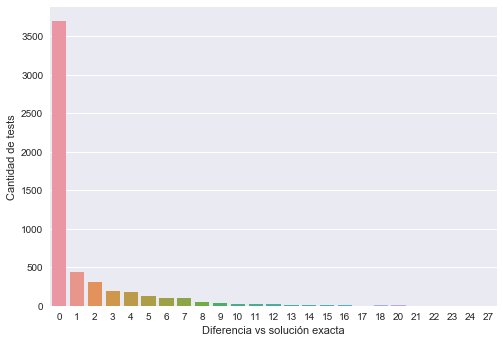
\includegraphics[scale=0.6]{img/accuracy-greedy.png}
\end{center}

A simple vista, en promedio, la heurística parece bastante precisa. De base podemos ver que el enfoque es efectivo para resolver el algoritmo, aunque no necesariamente suficiente. De estas pruebas pudimos extraer los siguientes indicadores:

\begin{center}
    \begin{tabular}{ | l l |}
        \hline
        Porcentaje de resultados con error & 30.98\% \\ \hline
        Error máximo & $max = 27$ \\ \hline
        Error promedio & $\mu = 1.229$ \\ \hline
        Desviacion estandar & $\sigma = 2.67$ \\
        \hline
    \end{tabular}
\end{center}

Como podemos ver, la heurística golosa de por sí no es tan exacta, aunque en promedio los errores son muy menores. Si miramos especificamente los casos patológicos del enfoque goloso:

TODO GRAFICO GREEDY PATOLOGICO ACA

TODO INDICADORES GREEDY PATOLOGICO ACA

Aquí podemos ver más claro los peores casos del algoritmo.

\subsection*{Heurística de búsqueda local}

\begin{center}
    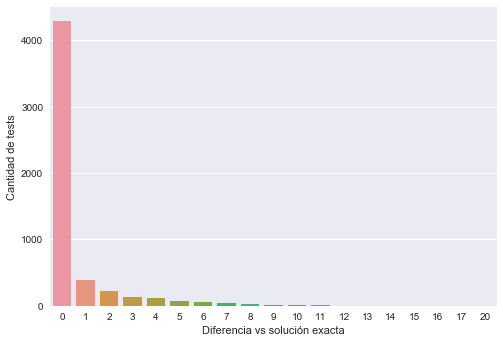
\includegraphics[scale=0.6]{img/accuracy-local.png}
\end{center}

Al aplicar una búsqueda local sobre la metodología greedy, podemos ver una amplia mejoría de los resultados obtenidos. La misma se evidencia mejor en los indicadores:

\begin{center}
    \begin{tabular}{ | l l |}
        \hline
        Porcentaje de resultados con error & 19.97\% \\ \hline
        Error máximo & $max = 20$ \\ \hline
        Error promedio & $\mu = 0.615$ \\ \hline
        Desviacion estandar & $\sigma = 1.698$ \\
        \hline
    \end{tabular}
\end{center}

En promedio, el error cae por debajo de 1, y la cantidad de casos con resultado exacto aumenta significativamente. Sin embargo, sigue habiendo varios errores, incluyendo algunas diferencias grandes.

TODO GRAFICO LOCAL PATOLOGICO ACA

TODO INDICADORES LOCAL PATOLOGICO ACA

\subsection*{Metaheurística GRASP}

Al analizar la precisión de GRASP, tuvimos que tener en cuenta los parámetros de la metaheurística: el porcentaje de los nodos considerados y la cantidad de iteraciones aleatorias. La combinatoria de estos dos parámetros es muy grande, así que decidimos mostrar solo algunos de los valores que consideramos representativos de las tendencias generales:

\begin{center}
    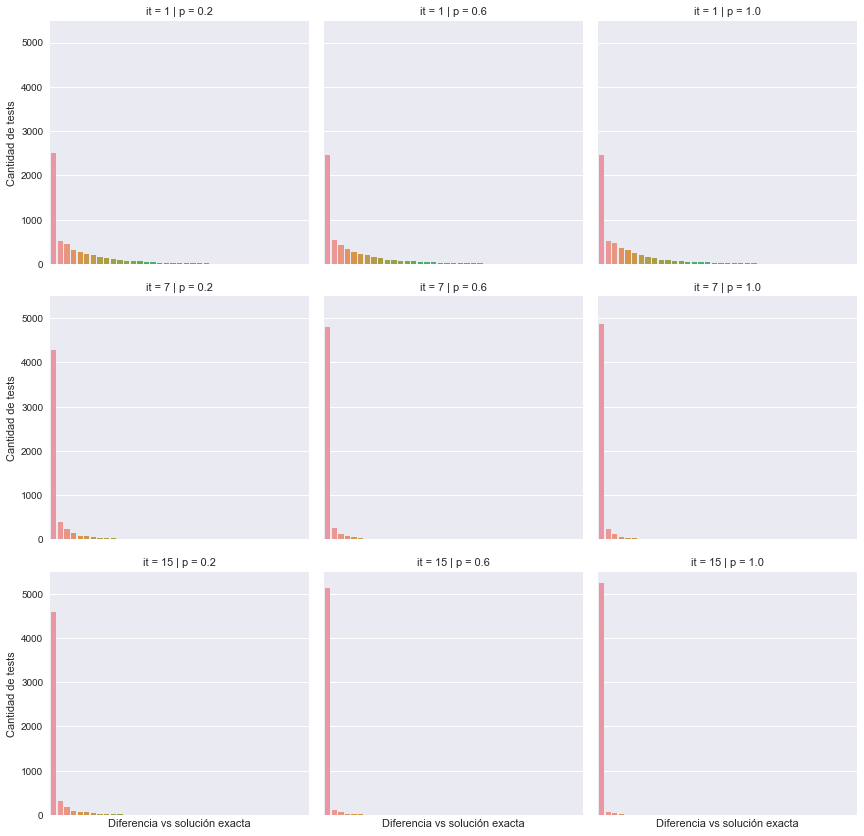
\includegraphics[scale=0.6]{img/accuracy-grasp-3x3.png}
\end{center}

Si bien este gráfico no permite un análisis muy profundo, muestra una tendencia básica: mientras más iteraciones se realizan, más errores se depuran, y la solución se aproxima más al resultado exacto.

\begin{center}
    \begin{tabular}{ | c | c | c | c | c | c |}
        \hline
        \% de nodos considerados & Iteraciones & \% de resultados con error & max & $\mu$ & $\sigma$ \\ \hline
         & 1 & 53.11\% & 39 & 3.046650 & 4.774386 \\ \cline{2-6}
        0.2 & 7 & 20.06\% & 27 & 0.617279 & 1.740223 \\ \cline{2-6}
         & 15 & 14.33\% & 16 & 0.391491 & 1.299830 \\ \hline
         & 1 & 54.02\% & 32 & 3.046091 & 4.679572 \\ \cline{2-6}
        0.6 & 7 & 10.34\% & 16 & 0.256764 & 1.014885 \\ \cline{2-6}
         & 15 & 4.22\% & 9 & 0.087330 & 0.528601 \\ \hline
         & 1 & 54.15\% & 46 & 3.003359 & 4.645715 \\ \cline{2-6}
        1 & 7 & 9.31\% & 12 & 0.212726 & 0.875136 \\ \cline{2-6}
         & 15 & 2.41\% & 9 & 0.052435 & 0.432504 \\
        \hline
    \end{tabular}
\end{center}

Mirando un poco más de cerca los datos obtenidos, se ve de manera mucho más clara en qué influye cada parámetro. En particular, podemos destacar un par de cosas

\begin{enumerate}
	\item el factor aleatorio de GRASP puede derivar en resultados menos fiables que usando una heurística golosa simple o con búsqueda local;
	\item si bien el porcentaje de nodos considerados influye en la tasa de error, la cantidad de iteraciones realizadas tiene un impacto mucho más visible, y es lo que permite a GRASP obtener mejores resultados que greedy, utilizando el aspecto random de manera ventajosa en lugar de generar casos patológicos;
	\item más allá de lo recíén dicho, la cantidad de iteraciones sigue una suerte de ley de retornos decrecientes, y aumentar la cantidad de repeticiones linealmente no genera resultados linealmente mejores, ya que las instancias aleatorias comienzan a repetirse
\end{enumerate}

Entre estos casos particulares, los parámetros que mejores resultados brindan son $p = 1$ e $it = 15$. Muy cerca de estos resultados se encuentra $p = 0.6$ e $it = 15$.

A modo de comparación con las pruebas realizadas en la sección de la metaheurística, probamos los parámetros particulares que fueron entregados con el ejecutable de este TP: $p = 0.6$ e $it = 50$.

\begin{center}
    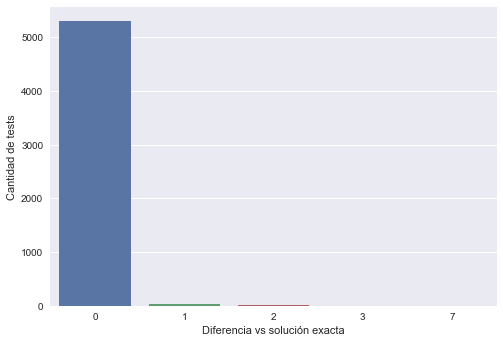
\includegraphics[scale=0.6]{img/accuracy-grasp50.png}

    \begin{tabular}{ | l l |}
        \hline
        Porcentaje de resultados con error & 1.04\% \\ \hline
        Error máximo & $max = 7$ \\ \hline
        Error promedio & $\mu = 0.0166$ \\ \hline
        Desviacion estandar & $\sigma = 0.189$ \\
        \hline
    \end{tabular}
\end{center}

Como se puede notar, el resultado es mucho más preciso que algunos de los casos mostrados anteriormente. Es más, en este caso, aumentar las iteraciones de 15 a 50 (resultando en más del triple del tiempo de ejecución) produjo una diferencia de calidad porcentualmente visible (se redujeron los errores a menos de la mitad, con mucho menor promedio y desviación).

Sin embargo, en términos netos, la diferencia no es tanta, ya que con muchas menos iteraciones la heurística estaba generando buenos resultados. Es difícil cuantificar esta diferencia, ya que depende mucho de los casos de prueba provistos y de la precisión deseada, pero vale la pena mencionar que este aumento en tiempo de ejecución podría no ser valioso.

TODO CASOS PATOLOGICOS GRASP ACA

TODO COMPARACIONES DE TIEMPO ENTRE HEURISTICAS ACA